%
% thesis.tex
%
% Master's Thesis/Ph.D. Dissertation Template
% Clemson University
%

%
% The document guidelines say the font can be between 10pt and 12pt.
% Specify whatever you want it to be here.
%
\documentclass[10pt]{ClemsonThesis}

%
% Use any additional packages you might need
%
%% \usepackage{listings}
%% \usepackage{comment}
\usepackage{fancyhdr}
\usepackage{array,booktabs}
\usepackage{multirow}
\usepackage{graphicx}
\usepackage{caption}
\usepackage{subcaption}
\usepackage{comment}
\usepackage{appendix}
\usepackage{color}
\usepackage{balance}

%
% Make the document your own -- fill in these values to reflect the type of
% document you are writing.
%
\title{Theorizing the Author/Format Editor Relational Dynamic:  A Study
       of the Manual Manuscript Review Process at Clemson University}
\department{School of Computing}
\documentType{Dissertation Proposal}
\major{Computer Science}
\degree{Doctor of Philosophy}
\graduationMonth{Aug}
\graduationYear{2018}
\author{Yangyang He}
\committeeChair{Dr. Bart P. Knijnenburg}
\committeeMemberOne{Dr. Larry F. Hodges}
\committeeMemberTwo{Dr. Alexander Herzog}
%% optional (for Master's) \committeeMemberThree{Dr. John Doe}
%% optional \committeeMemberFour{Dr. Jane Doe}
%% optional \committeeMemberFive{Dr. Mary Doe}
%% optional \committeeMemberSix{Dr. Mark Doe}

%
% PDF Setup -- most of this you do not need to touch
%
\hypersetup{
    colorlinks,
    linkcolor={black},
    citecolor={black},
    filecolor={black},
    urlcolor={black},
    pdftitle={\theTitle},
    pdfauthor={\theAuthor},
    pdfsubject={\theDocumentType},
    pdfkeywords={Clemson University, \theDepartment, \theDocumentType, \theMajor, \theDegree},
    pdfstartpage={1},
}


%
% User-specified command definitions/redefinitions
%
%% \newcommand{\cplusplus}{{\rm C\raise.5ex\hbox{\small ++}}}
%% \newcommand{\num}[1]{\mbox{(\textit{#1})}}
%% \renewcommand{\ttdefault}{pcr}
%% \renewcommand\lstlistlistingname{List of Listings}
\pagestyle{fancy}
\lhead{Yangyang He}
\rhead{Dissertation Proposal}
\renewcommand{\headrulewidth}{0.4pt}
\renewcommand*\contentsname{Outline}

\begin{document}
%  ============================================================================
    \frontmatter % Begin front matter (pages are numbered with Roman numerals)
%  ============================================================================

    \maketitle          % Generate the title page
    \singlespacing                             % Single space the lists
    % !TeX root = disseration.tex
\chapter{Author's Publications on this topic}
\noindent The work in this document is partially based on the following related publications.
\begin{enumerate}
	\item \textbf{He, Y.} (2019): Recommending Privacy Settings for IoT. In 24th International Conference on Intelligent User Interfaces (IUI ’19 Companion), March 17--20, 2019, Marina del Ray, CA.
	
	\item \textbf{He, Y.}, Bahirat, P., Knijnenburg, B.P. (2018): A Data Driven approach to Designing for Privacy in Household IoT. ACM Transactions on Interactive Intelligent Systems (TiiS).
	
	\item Sanchez, O., Torre, I.,\textbf{ He, Y.}, Knijnenburg, B.P. (2018) A Recommendation Approach for User Privacy Preferences in the Fitness Domain. User Modeling and User-Adapted Interaction (UMUAI).
	
	\item Bahirat, P., \textbf{He, Y.}, Knijnenburg, B.P. (2018): Exploring Defaults and Framing effects on Privacy Decision Making in Smarthomes. Interactive Workshop on the Human aspect of Smarthome Security and Privacy, SOUPS 2018, Baltimore, U.S.A.
	\item Bahirat, P., \textbf{He, Y.}, Menon, A., Knijnenburg, B.P. (2018): A Data-Driven Approach to Developing IoT Privacy-Setting Interfaces. In 23th International Conference on Intelligent User Interfaces, 2018, Tokyo, Japan.
	
	
%	
%Following are other publications that I have during my Ph.D.
%	\item Liu, J., Shen, H., Yu, L., Narman, H.S., Zhai, J., Hallstrom, J.O., He, Y. (2018): Characterizing Data Deliverability of Greedy Routing in Wireless Sensor Networks. IEEE Transactions on Mobile Computing (TMC) 17, 543-559.
%	\item Ge, R., Feng, X., He, Y., Zou, P. (2017): The Case for Cross-Component Power Coordination on Power Bounded Systems. ICPP2016, Philadelphia, PA, USA
%	\item Zhai, J., He, Y., Hallstrom, J.O. (2015): A Software Approach to Protecting Embedded System Memory from Single Event Upsets. EWSN2015, Porto, Portugal.
%	\item He, Y., Du, Y., Hughes, S., Zhai, J., Hallstrom, J.O., Sridhar, N. (2015): DESAL$^\beta$ : A Framework For Implementing Self-stabilizing Embedded Network Applications. International Internet of Things Summit, pp. 307-312. Springer, Cham, 2015.
%	\item Ruffing M., He Y., Kelly, M., Hallstrom, J.O., Olariu, S., Weigle, M.C. (2014): A Retasking Framework for Wireless Sensor Networks. Military Communications Conference (MILCOM), 2014 IEEE 1066-1071.
\end{enumerate} \clearpage
    \tableofcontents \clearpage                % Generate the Table of Contents
    %\addtotoc{List of Tables}{\listoftables}   % Generate the List of Tables
    %\addtotoc{List of Figures}{\listoffigures} % Generate the List of Figures
    %% \addtotoc{List of Listings}{\lstlistoflistings}
    
    \doublespacing % Text should be double spaced
	\addtotoc{Abstract}{\chapter*{Abstract}
The rapidly accelerating growth of these Internet of Things (IoT) technologies brings huge social and economic impact in many fields. However, the rise of IoT also comes with a number of privacy risks, including facilitation of the collection of large amounts of consumer data, processing and storing the data in ways unexpected by the consumer, and privacy and security breach.

Prior research has shown that privacy issues are the underlying obstacles to the adoption of social and mobile technologies. Privacy concerns have been identified as an important barrier to the growth of IoT. This is also true when it comes to the domain of setting privacy for IoT devices. The user interface for setting privacy preference of present IoT device is imperfect even for a smartphone, not to mention the complexity of manually setting privacy preferences for numerous different other IoT devices. Hence, there is a demand to solve the following, urgent research question: How can we help users simplify the task of controlling privacy setting for IoT devices in a user-friendly manner, so that they can make good privacy decisions?

Existing solutions to this problem in other domains involve giving users more control over, and information about the privacy settings provided by the systems as well as privacy nudges. However, neither of them work well in the IoT domain. Providing transparency and control does give users the freedom of managing their privacy in IoT according to their own privacy decisions, but privacy decision making is often not rational. Thus, such extra transparency and control may increase the difficulty of setting appropriate privacy for users. Privacy nudges are usually implemented in the form of prompts, which will create constant noises given that the IoT systems usually work in the background. At the same time, they lack the personalization to the inherent diversity of users’ privacy preferences and the context-dependency of their decisions.

To solve these problems in the IoT domain, a more fundamental understanding of the logic behind IoT users' privacy decisions in different IoT contexts is needed. We therefore conducted a series of studies to contextualize the IoT users' decision making characteristics, and designed a set of privacy-setting interfaces to help them manage their privacy settings in various IoT contexts based on the deeper understanding of users' privacy decision behaviors. 

In this proposal, we first present three studies on recommending privacy settings for different IoT environments, namely general/public IoT, household IoT, and fitness IoT, respectively. We developed and utilized a `` data-driven" approach in these three studies -- We first use statistical analysis and machine learning techniques on the collected user data to gain the underlying insights of IoT users' privacy decision behavior; and then create a set of ``smart" privacy defaults/profiles based on these insights. Finally, we design a set of interfaces to incorporate these privacy default/profiles. Users can apply these smart defaults/profiles by either a single click or by answering a few related questions.

Our current biggest limitation for such ``data-driven" approach is that we did not test any of the presented interfaces, so we do not know what level of complexity (both in terms of the user interface and the in terms of the profiles) is most suitable. Thus for my proposed work, I will address this limitation by discussing our proposed study to evaluate the new interfaces of recommending privacy-settings for household IoT. Our research can benefit the IoT users, manufacturers, and researchers, privacy-setting interface designers and anyone who has or want to adopt IoT devices.
}  % Generate the abstract
	
	%  ===========================================================================
	\mainmatter % Begin main matter (pages are numbered with Arabic numerals)
	%  ===========================================================================

    
    \setcounter{page}{1}
    % !TeX root = proposal.tex
\chapter{Motivation}\label{chapter:intro}
 
During the last two decades, computers have evolved into intricate personal tracking devices such as smart phones, smart watches, and fitness trackers. At the same time, computers and communication technologies are being embedded in appliances such as TVs, refrigerators, light fixtures and thermostats to create `smart home' environments. Finally, public sensing devices track us as we move about the built environment. By using all kinds of sensors, such as cameras, microphones, GPS, accelerometers, even the simplest of appliances are able to gain knowledge of its surrounding and their users. These connected devices, exchange data with each other, and further interact with our day-to-day activities. It is no longer surprising that our smart refrigerator knows what food is stored inside it and notify us that we need to buy groceries when we start our cars as we go back home from work. These smart connected devices are arguably revolutionizing our everyday life.

As forecast by Gartner~\cite{van_der_meulen_gartner_nodate}, the total number of 21 billion IoT devices will be in use by 2020. Cisco also predicts the global IoT market will be \$14.4 trillion by 2022. This rapidly accelerating growth of these Internet of Things (IoT) technologies brings a wealth of opportunities as well as risks. 

When users are considering adopting new IoT devices, they want to take the benefit of using those smart connected electronic devices by sharing and disclosing certain personal information to get a more personalized experience. However, such disclosed information could be accessed by other smart devices owned by themselves, other people, organizations, government, or some third-parties with good or bad purpose, which will result in unknown privacy risks to the users. A few research has shown that privacy issues are the underlying obstacles to the adoption of social and mobile technologies~\cite{}. Privacy concerns have been identified as an important barrier to the growth of IoT.

Most Internet users take a pragmatic stance when they have to make choices on what information that they want to disclose. They implicitly use a method called \textit{privacy calculus} to process their information disclosure decisions. They compare the perceived risks and anticipated benefit, and make decisions based on this risk-benefit analysis.

However, as the diversity of IoT devices increases, it becomes more and more difficult to keep up with the many different ways in which data about ourselves is collected and disseminated. Although generally users care about their privacy, few of them in practice find time to read the privacy policies or the privacy-settings carefully that are provided to them. There are several reasons for this problem: i) Users will pay more attention to the benefit than potential risks from using IoT devices or services. ii) The privacy policies are too long, or the privacy setting of such devices are too complicated, making users irritated to finish reading/setting them. iii) As the number IoT devices rapidly increases, the numbers and options of privacy setting for all the IoT devices will also increase exponentially. This privacy-setting choice overload makes it difficult for IoT users to correctly and precisely make their decision to express their true demands. 

In addition, the user interface for setting privacy preferences of present IoT devices is imperfect even for a smartphone, not to mention the complexity of manually setting privacy preferences for numerous different other IoT devices. Hence, there is an urgent demand to solve the following research question: 

\textbf{How can we help users simplify the task of controlling privacy setting for IoT devices in a user-friendly manner, so that they can make good privacy decisions?} This question can be further divided into two sub-questions: 1). Can we recommend them the appropriate IoT privacy-setting according to their decision making characteristics? )2. How do they feel about the new privacy-setting recommendation interface that we made?

In this proposal, we try to solve the main research question:
\begin{enumerate}
	\item In Chapter~\ref{chapter:acceptability}, we present a preliminary survey study that we conducted by interviewing with potential IoT users. By doing this, we try to gain deeper insight on the acceptability of IoT systems, which will be helpful and supportive to our following investigation to the decision-making process of IoT users when they share their personal data with differernt general public IoT devices. This will further affect how we design the privacy-setting interface and recommend privacy-settings for the users.
	
	\item In Chapter~\ref{chapter:generalIoT}, we demonstrate our existing work on recomming privacy preferences for general IoT. For this study, we leveraged data collected by Lee and Kobsa~\cite{lee2016understanding}, which asked 200 participants about their intention to allow or reject the IoT features presented in 14 randomized generated general public IoT usage scenarios. The scenarios have 5 manipulable parameters: `Who', `What', `Where', `Reason', and `Persistence'. We first apply statistical analysis on the dataset to determine the effect of each scenario parameter on users' decisions to allow the general IoT scenarios. Based on this statistical analysis, we design an ``layered'' intelligent user interface to reduce the complexity of manually setting privacy preferences for IoT. To further simplify the task of manully setting privacy preferences, we next use machine learning techniques to predict users' decisions based on the scenario parameters. By using Weka Java library, I develop 5 differernt machine learnign algorithms to cluster the participants and create a number of ``smart profiles''  accordingly. Each ``smart profile'' is a group of pre-set privacy setting preferences that users can apply by a single click. We present the detailed explanation of all the ``smart profiles''  to the users so that they can easily choose the one that are most suitable for them.
	
	\item In Chapter~\ref{chapter:householdIoT}, we expand 
	
	\item In Chapter~\ref{chapter:evaluation} I discuss my proposed study to evaluate the new interface of recommending privacy-settings for household IoT.
\end{enumerate}







    % !TeX root = proposal.tex
\chapter{Motivation}\label{motivation}

% Privacy is a big issue of adoption of new IoT technologies
Privacy issues are the underlying obstacles to the adoption of social and mobile technologies. Privacy concerns have been identified as an important barrier to the growth of Internet of Things. 

% privacy paradox
When the users are considering adopting the new IoT devices, they want to take the benefit of using those smart connected electronic devices by sharing and disclosing their certain personal information to get more personalized experience. However, such dis-closured information could be accessed by other smart devices owned by themselves, other people, organizations, government, or some third-parties with good or bad purpose, which will result in unknown risks to the users. Users have to make choices on what information that they want to disclose.

Most Internet users take a pragmatic stance on information disclosure. They implicitly use a method called \textit{privacy calculus} to process their information disclosure decisions. They compare the perceived risks and anticipated benefit, and make decisions based on this risk-benefit analysis.

However, as the increase of the diversity of IoT devices, it becomes more and more difficult to keep up with the many different ways in which data about ourselves is collected and disseminated. Although generally, users care about their privacy, few of them in practice find time to read the privacy policies or play around the privacy setting options that provided to them. There are several reasons leading to this problem: i) Users will think more of the benefit they will enjoy if they use the IoT devices or services than the potential risks if they disclose their information. ii) The privacy policies is too long, or the privacy setting of such devices are too complicated, making users irritated to finish reading/setting them. iii) As the rapid increment of numbers of IoT devices, the numbers and options of privacy setting for all the IoT devices are also increasing exponentially. This privacy-setting choice overload makes it difficult for IoT users to correctly and precisely make their decision to express their true demands. Thus, the main research question I propose to answer in my dissertation proposal is thus:


\textbf{How can we help users simplify the task of controlling privacy setting for IoT devices in a user-friendly manner, so that they can make good privacy decisions?}

To answer this research question, we first conduct a preliminary user study based on interviews with potential users to understand the acceptability of IoT systems and devices. We interviewed 10 users with the demographics shown in Table~\ref{tab:demographics1}. The interviews are approximately 30-50 minutes in length and covered a wide range of open questions related to IoT. These questions need participants to input their personal preferences about technology and self-perceived tech savviness. We first recorded the entire conversation with the participants on the understanding that their anonymity was kept. The entire recorded conversation was then transcribed manually. We also tried to take note of other interpersonal cues, e.g. body language, as well. Keywords, such as privacy and ease of use, have been focused on. During the analysis, we extracted the key statement from our interviews and used card sorting and affinity diagram techniques to group the specific statements.

\begin {table}
\caption {Participants Demographics} \label{tab:demographics1}
\vspace{8pt}
\begin{center}
	\begin{tabular}{|c|c|c|}
		\hline
		Age Range & \multicolumn{2}{c|}{ 21-35 }\\
		\hline
		& Male & 8 \\
		\cline{2-3}
		Gender    & Female & 2 \\
		\hline
		& Chinese & 2 \\
		\cline{2-3}
		Races 	  & Indians & 4 \\
		\cline{2-3}
		& Americans & 3 \\
		\cline{2-3}
		& Latin American & 1\\
		\hline
	\end{tabular}
\end{center}
\end {table}

Based on the results from our interviews, the factors that affect the acceptability of IoT devices can be summarized into following three aspects: Privacy, Usability, and Affordability. As shown in Figure~\ref{fig:AcceptingProcess}, while making the decision of whether to adopt the IoT technology, the users usually consider the trade-off between privacy and usability as against affordability. If the user's find that they are going to get better usability and privacy at a price that they can afford, they are more likely to go ahead and choose an IoT system. 

In a deeper level of usability, if the users find that the IoT systems will enhance their convenience, they will be more inclined to accept it. However, this is based on their perception of the actual utility of the automation provided by IoT. For example, if someone stays near a grocery store, he/she would tend to believe that there is not enough purpose for an IoT system when it comes to automatic ordering of the same grocery list online. 

The ability to control, which can also be seen as the capability to dominate over a technical entity and the extent to which this control can be exercised is one of the key aspects in determining the overall usability of the system. If the users think that they have a high level of control, they are likely to believe that the system has better usability.

In terms of privacy, the users primarily make judgements based on the trust they have on the brand/manufacturer and its public image. For example, one of our participants mentioned that he would trust apple when it comes to sharing of information, this participant had immense trust in Apple, based on some great reports recently published in newspapers. Hence, if they trust a brand with their data, they will have a better resolution of their privacy concerns, which would eventually lead to them accepting the technology. It is evident that the brand image will certainly play a key role in new users accepting the IoT technology.


\begin{figure}
	\centering
	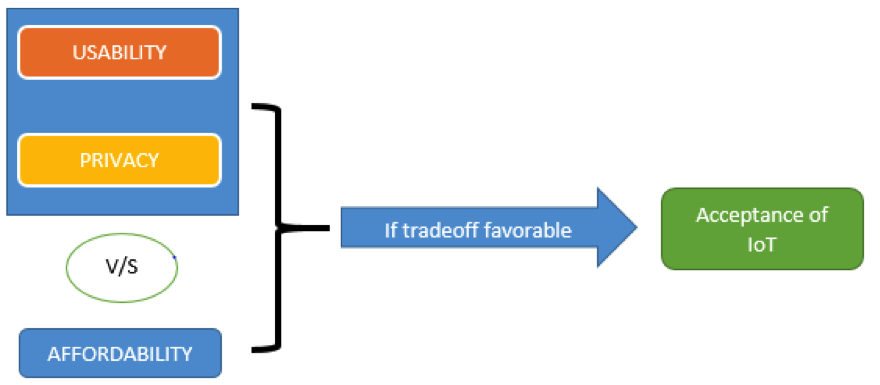
\includegraphics[width=0.6\columnwidth]{figures/AcceptingProcess.png}
	\caption{Process of accepting IOT as observed}
	\label{fig:AcceptingProcess}
\end{figure}

\section{IoT Privacy and Acceptability}
In this section, we present the ralation between privacy concerns and the acceptability of IoT systems/devices. The most important thing central to any IoT systems/devices is that there exists a constant sharing of information during the usage of such systems/devices. For example, in an environment of Household IoT, a refrigerator can sense what are stored inside it and can notify users when they need to refill the groceries. The entire IoT systems are highly relying on such data collections and sharing in order to provide the best possible experience to the users. However, users may find some of these data collections to be intrusive in nature. The perceived risks from the data collection and sharing can be the main obstacle that users would adopt IoT systems/devices. As one of the participants mentioned that, ``As long as the privacy issue can be managed and the companies can be responsible in keeping encrypted data so that it can't be easily hacked and all that. As long as everybody is respecting that privacy. I love it." Therefore, we consider privacy is one of the most important key factors which users would decide on, prior to accepting a new technology.

\subsection{Type of Information: \textit{What is collected/shared}}
There are various types of information can be collected/shared in an IoT systems, such as location, photos, voice, and videos. From our interview, we observe that different types of information have different levels of importance to the user. For example, a user may perceive different privacy-related concerns when his/her photos or videos are shared. Below is an excerpt from an interview which highlights the importance of what information is collected/shared:\\

\textit{I: ``So you are not ok with photo, video or voice?''\\}

\textit{P: ``Yes that's s pretty good generalization. Any data that is visuals of me photographs, voice, video, I would probably not want to store it.''\\}

\textit{I: ``About voice?''\\}

\textit{P: ``I mean, I understand that it is being stored to improve your algorithms but what if that was to get leaked.''\\}

typically, users are mostly uncomfortable with sharing their private data to other entities. ``May be sharing birthday or address, sharing those kind of data I'm not comfortable with". Another quote which proves the above point is "Maybe you can just share your common information, such as heartbeat data, sleeping data. But more critical, privacy data I don't want to share." They have their reservations against their private data being shared as it might threaten their security. Privacy information like date of birth and address helps in identifying the person and can be used to hack or rob the person. Therefore, we can say that people are worried about sharing their private information.

However, some participants expressed that some of their private data can be shared unless it is sensitive. One participant mentioned, "At this point I am not much concerned about my location being shared. I mean if somebody wants to find me they can find me anyhow without my location being shared. I don't mind location, I don't like personal messages or personal pictures, personal communication being shared. That bothers me, example my email has some social security or something.".

Another participant also mentioned, \textit {``Apart from photos, what other kind of information you like or don't like to be shared? Like saying something dirty to my girlfriend or something. That's okay like guy's being a guy. But if I am having really you know personal conversation about death of a loved one or something and we are trying to work out logistics or something. That's a problem for me. But for a regular conversation I am ok".} So the voice, seen as private data by many users, can be recorded or shared for some users.

It is intriguing that users were well aware of what type of information is collected/shared. This suggests that the designer of future IoT privacy-setting interfaces should provide the user separated options of allowing or denying data collecting/sharing for various types of information.

\subsection{Trust in IoT: \textit{Who is collecting, storing, and sharing my data?}}
Another aspect related to the IoT privacy we observed in our interviews is the \textbf{Trust}, the object of which is to whom users' informations are shared with. The object of trust from users can be varied in different contexts of IoT environments. For example, in general IoT environment, the objects can be an individual (e.g. your colleagues), an organization (e.g. your employer), the government and so on. While the user is in a Household IoT environment, his/her information may be first shared within all the connected IoT devices deployed in his/her home for various functionalities. Moreover, those smart IoT devices may further transfer users' information to their manufactures to store on a remote server (cloud) or even share them with the third-party for other purpose, such as advertisements and better recommendations. 

From our interview, we observed that the trust to the second-party or even the third-party also varies from user to user. One of the participants pointed out that, \textit{P: "For example, Apple in the news recently for refuting the FBI. FBI wanted in, Apple said we can't access these phone that actually turned me on to apple I previously used android. And the fact that they say they made their devices so secured that they can't even access them that really interests me. So yeah I am very concerned about it but I think now that I evolved into the Apple eco-system. I pretty much give apple everything because I trust them."}

Another example is:

\textit{I: ``Would you be alright if the manufacturer of those products collect your data and share with other organizations and provide more specific recommendation to you? Will you be OK with that?''\\}

\textit{P: ``I think I can be OK with that. Because the data this company collected are most time just shared or transfered to other companies who can analyze these data and get some information from these data.''\\}

\textit{I: ``Any company or any organization?''\\}

\textit{P: ``I think most are the manufacturers that I trust.''\\}

\textit{I: ``So you are OK with them to share your data?''\\}

\textit{P: ``Yes, I trust them.''\\}

It is evident from the conversation above that once established, trust can propagate from the second-party to the third-party via a "trust chain". As shown in Figure~\ref{fig:trustchain}, a "trust chain" is established when the organization we trust, deals with a third party organization which we are not aware about in the first place but still choose to trust. This kind of trust can be established only when there is a clear sight at the benefits that the user might get out of such a connection.

\begin{figure}
	\centering
	
\includegraphics[width=0.75\columnwidth]{figures/trustchain.pdf}
	\caption{Trust Chain}
	\label{fig:trustchain}
\end{figure}

Based on the interview results, users are well aware of who is collecting, storing, and sharing their data. They have a demand of controlling these data flows proceeded by different second-parties or third-parties. The designer of future IoT privacy-setting interfaces should solve the challenges of differing various second-parties and third-parties, and providing access control options available to users of different IoT contexts.

\section{IoT Usability and Acceptability}
We now present the effect that usability of the IoT devices has on the acceptability to IoT systems. We first describe the "convenience" and then move forward to discuss "control".

\subsection{Convenience and Usability}
The first most important aspect of usability is convenience. Convenience in case of IoT can be treated as the ease with which the IoT system offers funcitonality. Convenience can simply be a feedback which is provided by the temperature sensors in an household IoT system or the various recommendations provided by a recommender system in a way that it eases the shopping experience on e-commerce websites, such as \textit{Amazon.com}. One of the users was asked about how they would feel being in an IoT environment replied by saying, "Excited actually! When you describe that I don't know if that's sharing your same excitement but.. umm it actually is exciting to me because its so wonderfully convenient, so beautifully convenient." The same participant further went on saying "I love it. I mean it would be awesome to look at my phone right now and say 'oh! My door's unlocked'. Actually my brother has that, actually he can check his phone can look if the door locks. And it's really cool! You don't have to worry when you go out on a trip. Or you can control the A/C if you forgot. It's really cool."  It is clear from this statement that convenience of use of IoT systems is directly associated with the acceptability. Almost all of our participants pointed out the same thing in a similar way. The convenience offered through IoT systems by enabling the users with a common platform from where they can easily connect with their devices goes a long way in improving the overall usability of the systems and thereby impacts the acceptability of IoT in its totality. Usability for a few users also encompasses the aesthetics of any system which is evident from the statements made by participants.

\subsection{Being in Control and Usability}
Apart from convenience, the feeling of being in control of the system is also of equal importance. Another interesting aspect of control is that it is highly dependent on the information about the state of the system. Any individual will try to control something only when they are aware that it needs to be controlled or that it can be controlled. Therefore, being notified is primarily important before being able to control any aspect of the system. One of the participants when questioned about their opinion of overall usability of any device, mentioned enthusiastically that "I am excited by the idea that me being able to control what they want to do. I am less excited by the idea that them doing autonomously control what they want because some company told them to do it. Luckily the technology is so dumb right now. It's so linear, that it's not good at anticipating the things. But when it gets smarter, as long as it knew that I was an individual who would care, I think the same technology would allow you to totally automate your life but it would allow me to pick and choose which parts to automate". Even though users like a scenario of having everything automated, they still want to believe that they are in a position to control and are always aware of everything that the system is handling. It is evident from the comments that users want to keep absolute automation as a feature, but would probably completely rely on it when they have absolute confidence over its capability to handle things autonomously. A similar example in this regard would be the case of a pilot operating a commercial aircraft who would be prefer it more if the airplane were on autopilot while cruising. Although, he would also like to have the system informing him about the vital stats of the airplane while it's on autopilot. He would rather rely on his/her skills during landing and take-off of the aircraft. Lack of confidence in automated systems during decisive moments is a common trait found in human beings which in this case is clearly exhibited by the pilot.

\subsection{Being Notified and Being in Control}
"Control" can be the complete manual control of the system or it can be a situation where the user is notified regarding something which can be changed or altered subject to manual intervention. This is basically the system saying that it has an affordance which the user can utilize to better suit his/her convenience. In such a situation, the notification system (perhaps an application for IoT installed on the user's tablet) forms an interface between the machine and the user which serves as a medium to control the degree of automation. The entire idea behind having such an interface is to provide the user with control without compromising convenience. This phenomenon is depicted in the figure~\ref{fig:interface}.
\begin{figure}
	\centering
	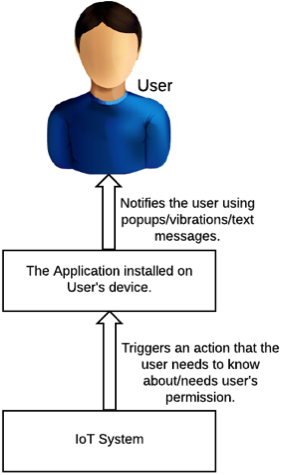
\includegraphics[width=4cm, height=6.3cm]{figures/interface.png}
	\caption{An interface for providing the user with "control"}
	\label{fig:interface}
\end{figure}

The assumption here is that the user is being notified about the several important aspects of the system. Being notified even after allowing something to take place is a requirement prevalent among many participants. One of the participants explicitly mentioned he would like periodic reminders about what is being recorded. This leads us to another interesting aspect of such a scenario which is the 'trust'. We assume that the user trusts the feedback from the system. The notification is perceived by the user as a kind of feedback and this leads to an impression of control in the user's mind where he/she is the master and the system is the apprentice. We think this situation is paramount in establishing trust and all participants desired it.

    % !TeX root = proposal.tex
\chapter{Work Completed}
In this chapter, we present the work completed to date in the areas of designing for privacy for general IoT and Household IoT.

\section{A Data-Driven Approach to Developing IoT Privacy-Setting Interfaces}
In this section, we present the data-driven design, the dataset that we use, the inspection of users' behaviors using statistical analyses, prediction of users' behaviors using machine learning techniques, and the privacy-setting prototypes that we create based on both statistical and machine learning results.

\subsection{Data-driven design}
What design process allows us to develop a usable privacy-setting interface for IoT? The development of usable privacy interfaces commonly relies on user studies with existing systems. However, this method is not possible in our IoT control scenario, because the Intel control framework has yet to be implemented~\cite{chow2015hci}. We therefore develop and employ a \emph{data-driven design} methodology, leveraging an existing dataset collected by Lee and Kobsa~\cite{lee2016understanding}, who asked users whether they would allow or deny IoT devices in their environment to collect information about them. We use this dataset in two phases. 

In our first phase, we develop a ``layered'' settings interface, where users make a decision on a less granular level (e.g., whether a certain recipient is allowed to collect their personal information or not), and only move to a more granular decision (e.g., what types of information this recipient is allowed to collect) when they desire more detailed control. This reduces the complexity of the decisions users have to make, without reducing the amount of control available to them. We use statistical analysis of the Lee and Kobsa dataset to decide which aspect should be presented at the highest layer of our IoT privacy-setting interface, and which aspects are relegated to subsequently lower layers.

In our second phase, we develop a ``smart'' default setting, which preempts the need for many users to manually change their settings~\cite{smith2013choice}. However, since people differ extensively in their privacy preferences~\cite{olson2005study}, it is not possible to achieve an optimal default that is the same for everyone. Instead, different people may require different settings. Outside the field of IoT, researchers have been able to establish distinct clusters or ``profiles'' based on user behavioral data~\cite{knijnenburg2013dimensionality, olson2005study, wisniewski2017making}. We perform machine learning analysis on the Lee and Kobsa dataset to create a similar set of ``smart profiles'' for our IoT privacy-setting interface.

The remainder of this paper is structured as follows: We first summarize previous work on privacy in IoT scenarios, and describe the structure of the Lee and Kobsa~\cite{lee2016understanding} dataset. We then \emph{inspect} users' behaviors using statistical analysis. Next, we \emph{predict} users' behaviors using machine learning methods. We subsequently present a set of prototypes for an IoT privacy-setting interface. Finally, we conclude with a summary of our proposed procedure and the results of our analysis.

\subsection{Dataset}
This study is based on a dataset collected by Lee and Kobsa~\cite{lee2016understanding}. A total of 2800 scenarios were presented to 200 participants (100 male, 99 female, 1 undisclosed) through Amazon Mechanical Turk. Four participants were aged between 18 and 20, 75 aged 20--30, 68 aged 30--40, 31 aged 40--50, 20 aged 50--60, and 2 aged $>$ 60. 

Each participant was presented with 14 scenarios describing a situation where an IoT device would collect information about the participant. Each scenario was a combination of five contextual parameters (Table~\ref{tab:parameter}), manipulated at several levels using a mixed fractional factorial design that allowed us to test main effects and two-way interactions between all parameters.

For every scenario, participants were asked a total of 9 questions. Our study focuses on the \textbf{allow/reject} question: ``If you had a choice to allow/reject this, what would you choose?'', with options ``I would allow it'' and ``I would reject it''. We also used participants' answers to three attitudinal questions regarding the scenario:
\begin{itemize}
	\item \textbf{Risk:} How risky or safe is this situation? (7pt scale from ``very risky'' to ``very safe'')
	\item \textbf{Comfort:} How comfortable or uncomfortable do you feel about this situation? (7pt scale)
	\item \textbf{Appropriateness:} How appropriate do you consider this situation? (7pt scale)
\end{itemize}

\begin{table*}
	\caption{Parameters used in the experiment. Example scenarios: \\\emph{``A device of a friend records your video to detect your presence. This happens continuously, while you are at someone else's place, for your safety.''}\\\emph{``A government device reads your phone ID to detect your identity. This happens once, while you are in a public place (e.g. on the street), for health-related purposes.''}}
	\label{tab:parameter}
	\begin{tabular}{l | l}
		\hline
		\textbf{Parameter} & \textbf{Levels} 	 \\ \hline
		\multirow{7}{9.5em}{Who\\\rule{0pt}{4ex}\emph{The entity collecting the data}}		& 1. Unknown \\
		& 2. Colleague							 \\
		& 3. Friend								 \\
		& 4. Own device							 \\
		& 5. Business 							 \\
		& 6. Employer 							 \\
		& 7. Government							 \\ \hline
		\multirow{24}{9.5em}{What\\\rule{0pt}{4ex}\emph{The type of data collected and (optionally) the knowledge extracted from this data}}	& 1. PhoneID	\\	
		& 2. PhoneID$>$identity				\\	
		& 3. Location						\\	
		& 4. Location$>$presence			\\	
		& 5. Voice							\\	
		& 6. Voice$>$gender					\\	
		& 7. Voice$>$ age 					\\	
		& 8. Voice$>$identity				\\	
		& 9. Voice$>$presence				\\	
		& 10. Voice$>$mood					\\	
		& 11. Photo							\\	
		& 12. Photo$>$gender				\\	
		& 13. Photo$>$age  \\
		& 14. Photo$>$identity	 \\
		& 15. Photo$>$presence 	 \\
		& 16. Photo$>$mood 	 \\
		& 17. Video	 \\
		& 18. Video$>$gender	 \\
		& 19. Video$>$age 		 \\
		& 20. Video$>$presence 	 \\
		& 21. Video$>$mood 	 \\
		& 22. Video$>$looking at	 \\
		& 23. Gaze	 \\
		& 24. Gaze$>$looking at	 \\ \hline
		\multirow{4}{9.5em}{Where\\\rule{0pt}{4ex}\emph{The location of the data collection}}	& 1. Your place		\\
		& 2. Someone else's place		\\				
		& 3. Semi-public place (e.g. restaurant) \\
		& 4. Public space (e.g. street) \\ \hline
		\multirow{6}{9.5em}{Reason\\\rule{0pt}{4ex}\emph{The reason for collecting this data}} & 1. Safety	\\
		& 2. Commercial						\\
		& 3. Social-related	\\
		& 4. Convenience \\
		& 5. Health-related \\
		& 6. None \\ \hline
		\multirow{2}{9.5em}{Persistence} & 1. Once \\
		& 2. Continuously \\ 
		\emph{Whether data is collected once or continuously} & \\ \hline
	\end{tabular}
\end{table*}

\subsection{Inspecting users' behaviors}
In this section we analyze how users' behavioral intentions to allow or reject the information collection described in the scenario are influenced by the scenario parameters. In line with classic attitude-behavior models~\cite{ajzen1977attitude}, we also investigate whether users' attitudes regarding the scenario---their judgment of risk, comfort, and appropriateness---mediate these effects. This mediation analysis~\cite{baron1986moderator} involves the following test:
\begin{itemize}
	\item \textbf{Test 1:} The effect of the scenario parameters (who, what, where, reason, persistence) on participants' attitudes (risk, comfort, appropriateness).
	\item \textbf{Test 2:} The effect of participants' attitudes on their behavioral intentions (the allow/reject decision).
	\item \textbf{Test 3:}  The effect of the parameters on behavioral intentions, controlling for attitudes.
\end{itemize}

If tests 1 and 2 are significant, and test 3 reveals a substantial reduction in conditional direct effect (compared to the marginal effect), then we can say that the effects of the scenario parameters on participants' behavioral intention are mediated by their attitudes. Moreover, if the conditional direct effect is (close to) zero, then the effects are fully (rather than partially) mediated.

\subsubsection{Scenario Parameters and Attitude}\label{subsec:attitude}
\textbf{ANOVA Test of Main Effects: }
To understand the effect of the scenario parameters on participants' attitudes, we created a separate \textit{linear mixed effects regression} (\textit{lmer}) model with a random intercept (to account for repeated measures on the same participant) for each dependent variable (risk, comfort, appropriateness), using the scenario parameters as independent variables. We employed a forward stepwise procedure, adding the strongest remaining parameter into the model at each step and comparing it against the previous model. Table~\ref{tab:anovaEffect} shows that all parameters except \textbf{where} have a significant effect on each of the attitudes.

\textbf{Post-hoc Comparisons: }
We also conducted Tukey post hoc analyses to better understand how the various values of each parameter influenced the attitudes. \textbf{Where} was excluded from these analyses, as it did not have an overall significant effect. Some key findings of these post hoc analyses are:

\begin{table}
	\centering
	\caption{Effect of scenario on attitudes. Each model builds upon and is tested against the previous.}
	\label{tab:anovaEffect}
	\begin{tabular}{ l | r | r | r}
		\hline
		Model &	$\chi^2$ &	$df$ & $p$-value \\ \hline
		$risk\sim(1|sid)$ &				 &			 &						\\ 
		+who &				315.37 &	6 &			$<$ .0001 		\\ 
		+what &			67.74 &		23 &		$<$ .0001 		\\ 
		+reason & 			15.65 &		5 &		.0079 			\\ 
		+persistence &		9.95 &		1 &		.0016 			\\ 
		+where	&			7.47 &		3 &		.0586 			\\ 
		+who:what &		166.47 &	138 &	.0050			\\
		\hline
		Model &	$\chi^2$ &	$df$ & $p$-value \\ \hline
		$comfort\sim(1|sid)$ & 			 &			&	 					\\
		+who &				334.06 &	6 &			$<$ .0001 		\\
		+what &			83.24 &		23 &		$<$ .0001 		\\
		+reason &			18.68 &		5 &			.0022 		\\
		+persistence &		14.73 &		1 &			.0001 		\\
		+where &			3.25 &		3 &			.3544 		\\ 
		+who:what &		195.07 &	138 &		.0001			\\
		\hline
		Model &	$\chi^2$ &	$df$ & $p$-value \\ \hline
		$appropriateness\sim(1|sid)$ &	 &		 &						\\
		+who &				315.77 &	6 &			$<$ .0001 		\\
		+what &			72.87 &		23 &		$<$ .0001 		\\
		+reason &			23.27 &		5 &			.0003 		\\
		+persistence &		8.97 &		1 &			.0027 		\\
		+where &			5.46 &		3 &			.1411 		\\
		+who:what &		214.61 &	138 &		$<$ .0001			\\ 
		\hline
	\end{tabular}
\end{table}

\textbf{Who:} Participants perceive more \emph{risk} when the recipient of the information is `unknown' than for any other recipient ($d$ range = [0.640, 1.450] and all $p$s~$<$~.001, except for `government': $d=0.286$, $p < .05$). `Government' is the next most risky recipient ($d$ range = [0.440, 1.190], all $p$s~$<$~.001). Participants consider their `own device' the least risky ($d$ range = [0.510, 1.450], all $p$s~$<$~.001). Similar patterns were found for \emph{comfort} and \emph{appropriateness}.

\textbf{Reason:} Participants were more \emph{comfortable} disclosing information for the purpose of `safety' than for any other reason except `health' ($d$ range = [0.230, 0.355], all $p$s~$<$~.05). They also believe that disclosing information for the purpose of `health' or `safety' is more \emph{appropriate} than for `social' or `commercial' purposes ($d$ range = [0.270, 0.310], all $p$s~$<$~.05).

\textbf{Persistence:} Participants were more \emph{comfortable}, found it more \emph{appropriate}, and less \emph{risky} to disclose their information `once' rather than `continuously' ($d = 0.146$, $p < .01$).

\textbf{What:} This parameter has a large number of values, so we decided to selectively test planned contrasts instead of post-hoc tests. We first compared different mediums (voice, photo, video) regardless of what is being inferred:
\begin{itemize}
	\item Participants were significantly more \emph{comfortable} with `voice' than `video' ($d = 0.260$, $p = .005$), and found `voice' less \emph{risky} ($d = -0.239$, $p = .005$) and more \emph{appropriate} ($d = 0.217$, $p = .015$) than `video'.
	\item Participants were significantly more \emph{comfortable} with `voice' than `photo' ($d=0.201$, $p = .007$) and found `voice' more \emph{appropriate} than `photo' ($d = 0.157$, $p$~$=$~$.028$). There was no significant difference in terms of \emph{risk} ($p = .118$).
	\item No differences were found between `photo' and `video' in terms of \emph{risk} ($p = .24$), \emph{comfort} ($p = .35$) and \emph{appropriateness} ($p = .26$).
\end{itemize}

We also compared different inferences (e.g. age, gender, mood, identity) across mediums. The following planned contrasts were significant (all others were not):
\begin{itemize}
	\item Participants were significantly more \emph{comfortable} ($d$~$=$~$0.363$, $p = .028$) and found it more \emph{appropriate} ($d = 0.371$, $p = .018$) to reveal their `age' rather than their `identity'.
	\item Participants were significantly more \emph{comfortable} ($d$~$=$~$0.363$, $p= .008$) and found it more \emph{appropriate} ($d = 0.308$, $p = .024$) to reveal their `presence' rather than their `identity'. 
\end{itemize}

\textbf{Interaction effects: }
We also checked for two-way interactions between the scenario parameters. The only significant interaction effect observed was between \textbf{who} and \textbf{what}. The last line of each section in Table~\ref{tab:anovaEffect} shows the results of adding this interaction to the model. Due to space concerns, we choose not to address the post-hoc analysis of the $7 * 24 = 168$ specific combinations of who and what.

\subsubsection{Attitude and Behavioral intention}
To test the effects of participants' attitudes on their allow/reject decision, we ran a \emph{generalized linear mixed effects regression} (\emph{glmer}) with a random intercept and a logit link function to account for the binary dependent variable.
We found significant effects of all the three attitudes on participants' allow/reject decision (see Table~\ref{tab:mediationANOVA}). Each 1-point increase in \textbf{risk} results in a 4.04-fold decrease in the odds that the scenario will be allowed ($p < .0001$). Each 1-point increase in \textbf{comfort} results in a 5.04-fold increase ($p < .0001$), and each 1-point increase in \textbf{appropriateness} results in a 3.47-fold increase ($p < .0001$).

\textbf{Mediation Analysis: }
The bottom half of Table~\ref{tab:mediationANOVA} shows the \emph{conditional} effects of the significant parameters (who, what, reason, persistance) on participants' allow/reject decision, controlling for attitude. \textbf{Who} and \textbf{what} are no longer significant; these effects are thus fully mediated by attitude. The effects of \textbf{reason} and \textbf{persistance} are still significant, but smaller than the marginal effects (i.e., without controlling for attitude, see Table~\ref{tab:marginalANOVA})---their $\chi^2$s are reduced by 12\% and 39\%, respectively. This means that the mediation effect was substantial in all cases. The final mediation model is displayed in Figure~\ref{fig:mediationAllow}.


\begin{table}
	\centering
	\caption{Effect of attitudes and scenario on allow/reject.}
	\label{tab:mediationANOVA}
	\begin{tabular}{ l | r | r | r | r }
		\hline
		Model & OR	&	\textbf{$\chi^2$} & $df$ & $p$-value 	\\ \hline
		$allow\sim(1 | sid)$ &	&		  &	    &				\\
		+risk &				0.25 &	1005.24  &    1 &		$<$ .0001 \\
		+comfort &			5.04 &	723.27  &     1 &		$<$ .0001 \\
		+appropriateness &	3.47 &	128.17  &	  1 & 		$<$ .0001 \\ \hline
		+who &					&	8.80	& 	  6 & 		.1851 	\\
		+what &					&	26.07 &	  	 23 &		.2976 	\\
		+reason &				&	19.33 & 	  5 & 		.0017	\\
		+persistence &			&	12.69 &	 	  1 & 		.0004 	\\
		\hline
	\end{tabular}
\end{table}

\begin{table}
	\centering
	\caption{Effect of scenario on allow/reject, \emph{not} controlling for attitudes.}
	\label{tab:marginalANOVA}
	\begin{tabular}{ l | r | r | r }
		\hline
		Model &	$\chi^2$ & $df$ & $p$-value 	\\ \hline
		$allow\sim(1 | sid)$ &		  	&	    &				\\
		+who &					221.36	& 	  6 & 		$<$ .0001 	\\
		+what &					78.55 &		  23 &		$<$ .0001 	\\
		+reason &				21.95 & 	  5 & 		  .0005		\\
		+persistence &			20.64 &		  1 & 		$<$ .0001 	\\
		\hline
	\end{tabular}
\end{table}

\begin{figure}
	\centering
	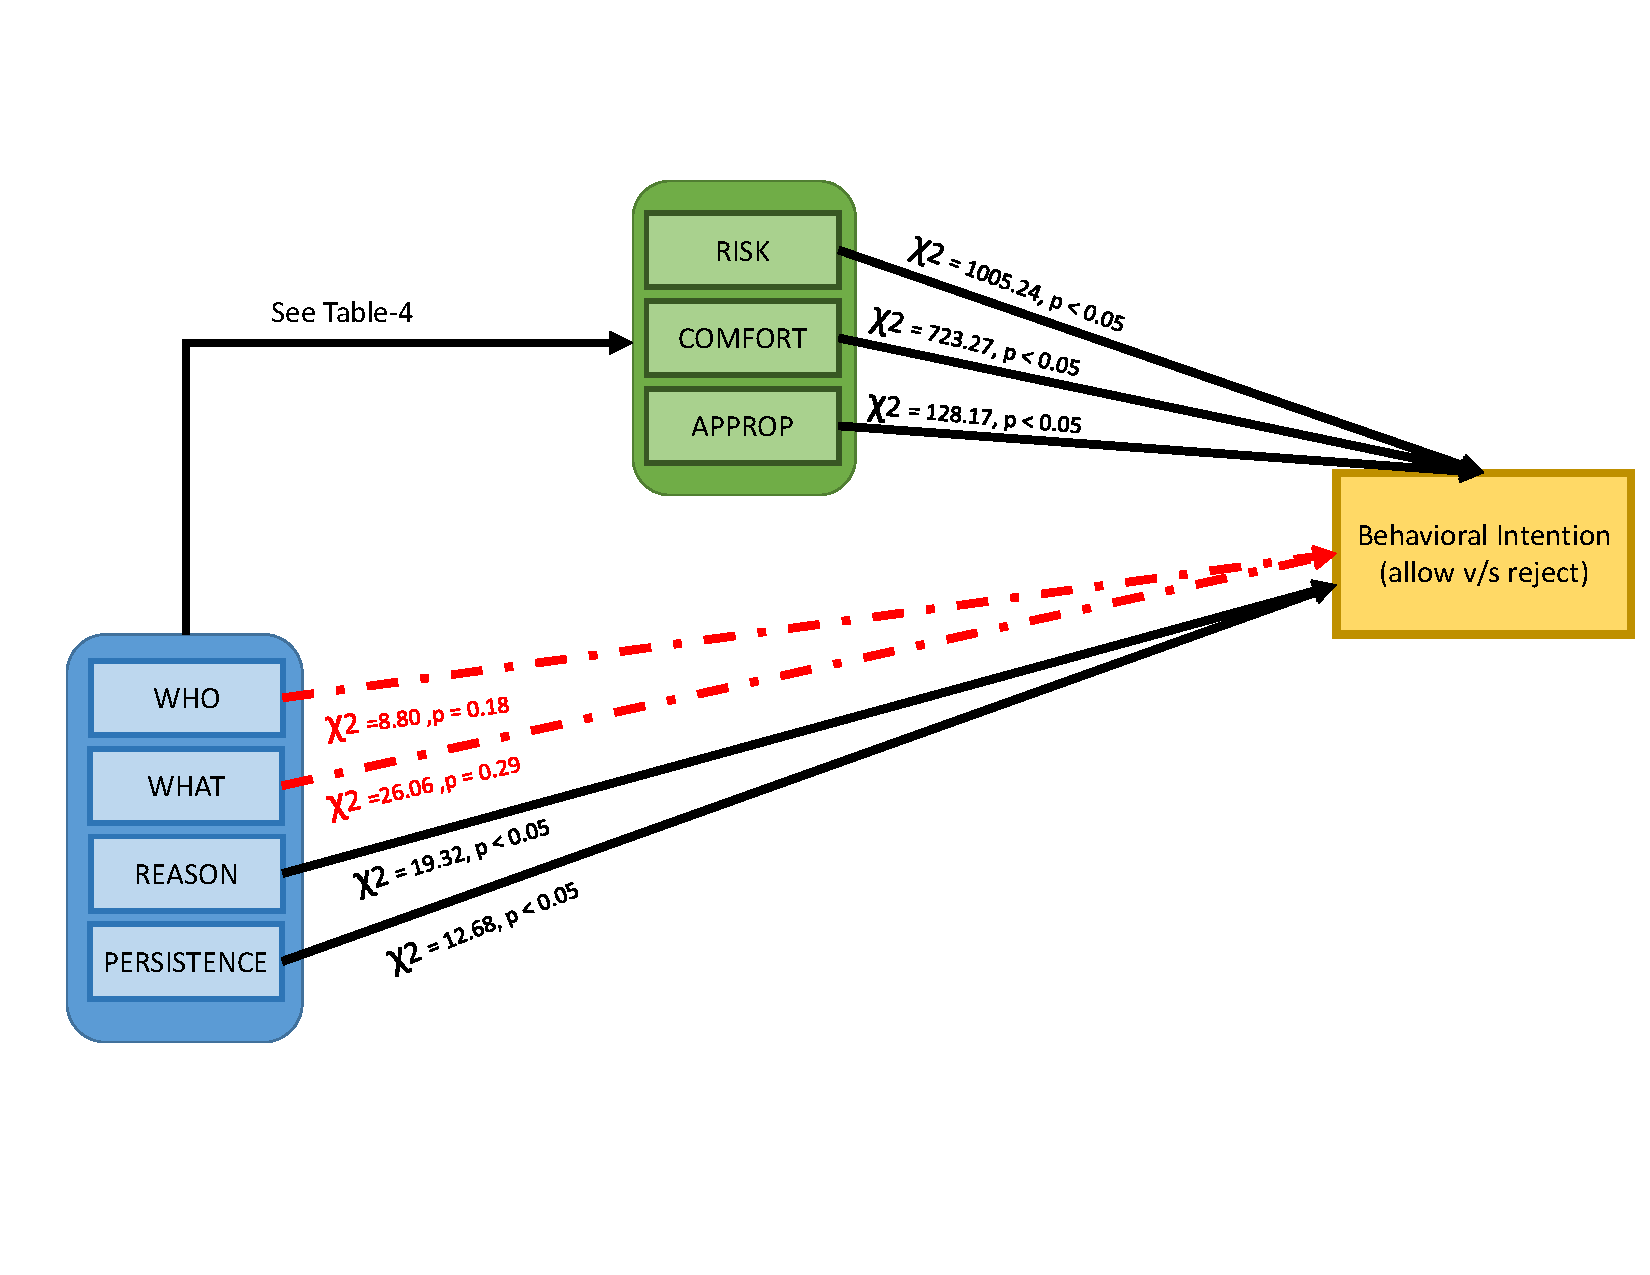
\includegraphics[width=0.45\textwidth]{figures/allow.pdf}
	\caption{Mediation model of the effect of scenario parameters on participants' intention to allow/reject the scenario, mediated by attitudinal factors}
	\label{fig:mediationAllow}
\end{figure}

\subsubsection{Discussion of Statistical Results}
Our statistical results show several patterns that can inform the development of an IoT privacy-setting interface. We find that \textbf{who} is the most important scenario parameter, and should thus end up at the top layer of our interface. People are generally concerned about IoT scenarios involving unknown and government devices, but less concerned about about data collected by their own devices. Mistrust of government data collection is in line with Li et al.'s finding regarding US audiences~\cite{li2017cross}.

\textbf{What} is the next most important scenario parameter, and its significant interaction with \textbf{who} suggests that some users may want to allow/reject the collection of different types of data by different types of recipients. Privacy concerns are higher for photo and video than for voice, arguably because photos and videos are more likely to reveal the identity of a person. Moreover, people are less concerned with revealing their age and presence, and most concerned with revealing their identity.

The \textbf{reason} for the data collection may be used as the next layer in the interface. Health and safety are generally seen as acceptable reasons. \textbf{Persistence} is less important, although one-time collection is more acceptable than continuous collection. \textbf{Where} the data is being collected does not influence intention at all. This could be an artifact of the dataset: location is arguably less prominent when reading a scenario than it is in real life.

Finally, participants' attitudes significantly (and in some cases fully) mediated the effect of scenario parameters on behavioral intentions. This means that these attitudes may be used as a valuable source for classifying people into distinct groups. Such attitudinal clustering could capture a significant amount of the variation in participants in terms of their preferred privacy settings, espcially with respect to the \textbf{who} and \textbf{what} dimensions.
    % !TeX root = proposal.tex
\chapter{Proposed Work}
In this chapter, we discuss our proposed work focusing on evaluating the user experience of the privacy-setting interface

To further explore this trade-off between parsimony and accuracy, and also to evaluate the usability of the proposed privacy-setting interface prototypes in~\cite{he2018data}, we are in a process of developing a user study to test these interface prototypes. This is going to be a between-subject study. All the participants will be recruited through Amazon Mechanical Turk. 

In this user study, we will manipulate two different independent variables to compare several default/profile solutions. The first one is the extend of default/profile's conservatives. We consider the default settings that with all disabled by default as the most conservative profile; and the default settings with all enabled by default as the most open profile, the `smart default' and `smart profiles' are considered to be in the middle. The other independent variable is the different levels of complexity for the settings interface. Hence 4x2=8 total experimental conditions (i.e., user interfaces) will be presented to the participants. The Dependent variable of our study will be the user experience of the system, including the satisfaction and trust to the company.

During the user study, the users will be first introduced the concept of the devices that appearing in the study, corresponding to the `Who' and `What' parameters of an IoT scenario. The introduction contains both figures, text, and audio information. After the introduction, the participant will be given an example scenario to further understand the context of our study. Attention checks will also be given here to make sure the participants have paid attention to the explanations.

After above procedures, one of the 8 user interfaces will be randomly chosen for each participants. Participants need to go through the whole interface to see if the preset privacy settings is suitable for them, and make necessary changes to accommodate their actual privacy demands. All these changes will be recorded to compared with the preset settings for further analysis purpose.

Next, the participants will be give a survey containing questions about three different aspects: \textit{Subjective System Aspects}, \textit{Personal Characteristics}, and \textit{Situational Characteristics}, as shown in Figure~\ref{fig:model}.

\begin{figure}
	\centering
	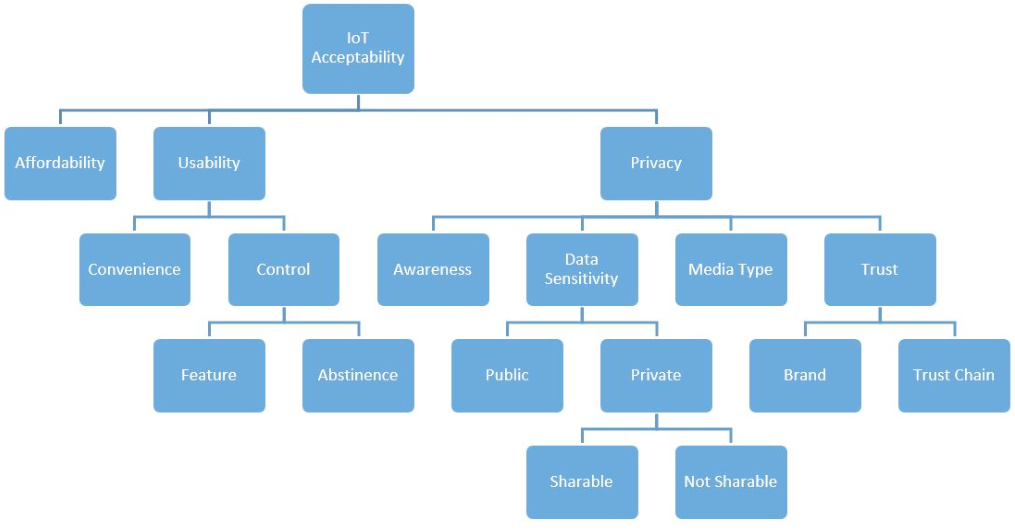
\includegraphics[width=0.48\textwidth]{figures/model.pdf}
	\caption{Accuracy of our clustering approaches}
	\label{fig:model}
\end{figure}

We expect to see a significant improvement for the `smart default' and `smart profile' interfaces in terms of system satisfaction and Trust over the baseline user interface (All-on or All-off). We will use statistics to analysis the effect of the independent variables on the subjective system aspects, and further mediation effect on the user experience. We also wonder how the personal characteristics ans situational characteristics affect the user experience. Finally, we will apply machine learning techniques to uncover deep insights of the results.
    % !TeX root = proposal.tex
\chapter{Related Work}
In this chapter, we discuss existing research on privacy-setting interfaces and on privacy prediction, and finally we discuss why we use a data-driven design to recommending privacy preference in IoT.

\section{Personalization in IoT Systems}
One of the key features of IoT environments is that they have a high potential for providing personalized services to their users~\cite{vallee2016personalization, etzion2014personalization, hemant2015internet}. For example, Russell et al.~\cite{russell2015personalization} use unobtrusive sensors and micro-controller to realize a human detection for further providing personalization in a scenario of a family making use of the IoT in their daily living. Henka et al.~\cite{henka2016personalizing} propose an approach to personalize services in (household) IoT using the Global Public Inclusive Infrastructure's~\cite{vanderheiden2011creating} preference set to describe an individual's needs and preferences, and then adapting a smart environment accordingly.

\section{Privacy in Personalized systems}
Researchers have shown that privacy can play a limiting role in users' adoption of personalized services~\cite{teltzrow_2004}.  For example, Awad and Krishnan~\cite{awad_2006} show that privacy concerns inhibit users' use of personalized services, and Sutanto et al.~\cite{sutanto_2013} demonstrated that privacy concerns can prevent people from using a potentially beneficial personalized application. Kobsa et al.~\cite{kobsa_2016} demonstrate that the personalization provider is an important determinant of users' privacy concerns.

Moreover, research has shown  users' willingness to provide personal information to personalized services depends on both the risks and benefits of disclosure~\cite{phelps_2000,ho_2006,hui_2006}, and researchers therefore claim that both the benefits and the risks meet a certain threshold~\cite{treiblmaier_2007}, or that they should be in balance~\cite{chellappa_2005}.

\section{Privacy in IoT}
The argument that using user-generated data for personalization can result in privacy concerns has also been made in IoT environments~\cite{worthy_trust_2016}. 
	One of the first examples in this regard was the work by, Sheng et al.~\cite{sheng_experimental_2008}, who showed that users of ``u-commerce'' services (IoT-driven mobile shopping) felt less inclined to use personalized (rather than non-personalized) u-commerce services, unless the benefits were overwhelming (i.e., providing help in an emergency).

In response, researchers have proposed frameworks with guidelines for evaluating the security and privacy of consumer IoT applications, devices, and platforms~\cite{perera_privacy-by-design_2016, loi_systematically_2017}. Most of these guidelines focus on minimizing data acquisition, storage, and collection sources. Along these guidelines, several researchers have proposed architectures that restrict unwanted access to users' data by IoT devices. For example, Davies et al. propose ``privacy mediators'' to the data distribution pipeline that would be responsible for data redaction and enforcement of privacy policies even before the data is released from the user's direct control~\cite{davies_privacy_2016}. Likewise, Jayraman et al.'s privacy preserving architecture aggregates requested data to preserve user privacy~\cite{jayaraman_privacy_2017}.

Other research has considered IoT privacy from the end-user perspective~\cite{feth_user-centered_2017}, both when it comes to research (e.g., Ur et al. investigated how privacy perceptions differ among teens and their parents in smart security systems installed in homes~\cite{ur_intruders_2014}) and design (e.g., Williams et al. highlight the importance of designing interfaces to manage privacy such that they are usable to the end users of IoT devices~\cite{williams2016perfect}, and Feth et al. investigated the creation of understandable and usable controls~\cite{feth_user-centered_2017}). The current paper follows this approach, by outlining a novel methodology for the development of usable and efficient privacy-setting interfaces and applying it to household IoT privacy management. 

\section{Existing privacy control schemes}
Smartphones give users control over their privacy settings in the form of prompts that ask whether the user allows or denies a certain app access to a certain type of information. Such prompts are problematic for IoT, because IoT devices are supposed to operate in the background. Moreover, as the penetration of IoT devices in our homes continues to increase, prompts would become a constant noise which users will soon start to ignore, like software EULAs~\cite{good2005spyware} or privacy policies~\cite{jensen2004privacy}.

Pejovic and Musolesi~\cite{Pejovic2014} presented the design and implementation of an efficient online learner that can serve as a basis for recognizing opportune moments for interruption. The design of the library is based on an in-depth study of human interruptibility. Comparatively, our work tries to find the most suitable privacy-setting profile for each user based on their privacy preference on different household IoT scenarios.

\section{Privacy-Setting Interfaces}
Beyond prompts, one can regulate privacy with global settings. The most basic privacy-setting interface is the traditional ``access control matrix'', which allows users to indicate which entity gets to access what type of information~\cite{sandhu1994access}. This approach can be further simplified by grouping recipients into relevant semantic categories, such as Google+'s \emph{circles}~\cite{watson12}. Taking a step further, Raber et al.~\cite{197908} proposed \emph{Privacy Wedges} to manipulate privacy settings. Privacy Wedges allow users to make privacy decisions using a combination of semantic categorization (the various wedges) and inter-personal distance (the position of a person on the wedge). Users can decide who gets to see various posts or personal information by ``coloring'' parts of each wedge. 

Privacy wedges have been tested on limited numbers of friends, and in the case of household IoT they are likely to be insufficient, due to the complexity of the decision space. To wit, IoT privacy decisions involve a large selection of devices, each with various sensors that collect data for a range of different purposes. This makes it complicated to design an interface that covers every possible setting~\cite{williams2016perfect}. A wedge-based interface will arguably not be able to succinctly represent such complexity, and therefore either be impossible, or still lead to a significant amount of information and choice overload. 

We propose a data-driven approach to solve this problem: statistical analysis informs the construction of a layered settings interface, while machine learning-based privacy prediction helps us find smart privacy profiles.


\section{Privacy Prediction}
Several researchers have proposed privacy prediction as a solution to the privacy settings complexity problem---an approach known as ``user-tailored privacy'' (UTP)~\cite{knijnenburg2017}. Systems that implement UTP first predict users' privacy preferences and behaviors based on their known characteristics. They then use these predictions to provide automatic default settings or suggestions in line with users' disclosure profiles, to educate users' about privacy features they are unaware of, to tailor the privacy-setting user interfaces to make it easier for users to engage with their preferred privacy management tools, or to selectively restrict the types of personalization a system is allowed engage in.

Most existing work in line with this approach has focused on providing automatic default settings. For example, Sadeh et al.~\cite{sadeh2009understanding} used a k-nearest neighbor algorithm and a random forest algorithm to predict users' privacy preferences in a location-sharing system, based on the type of recipient and the time and location of the request. They demonstrated that users had difficulties setting their privacy preferences, and that the applied machine learning techniques can help users to choose more accurate disclosure preferences. Similarly, Pallapa et al.~\cite{pallapa2014adaptive} present a system which can determine the required privacy level in new situations based on the history of interaction between users. Their system can efficiently deal with the rise of privacy concerns and help users in a pervasive system full of dynamic interactions.

Dong et al.~\cite{dong2016ppm} use a binary classification algorithms to give users personalized advice regarding their privacy decision-making practices on online social networks. They found that J48 decision trees provided the best results. Li and et al.~\cite{li2017cross} similarly use J48 to demonstrate that taking the user's cultural background into account when making privacy predictions improves the prediction accuracy. Our data stems from a culturally homogeneous population (U.S. Mechanical Turk workers), so cultural variables are outside the scope of our study. We do however follow these previous works in using J48 decision trees in our prediction approach.

We further extend this approach using \emph{clustering} to find several smart default policies (``profiles''). This is in line with Fang et al.~\cite{fang2010privacy}, who present an active learning algorithm that comes up with privacy profiles for users in real time. Since our approach is based on an existing dataset, our algorithm does not classify users in real time, but instead creates a static set of profiles `offline', from which users can subsequently choose. This avoids cold start problems, and does not rely on the availability of continuous real-time behaviors. This is beneficial for household IoT privacy settings, because users often specify their settings in these systems in a ``single shot'', leaving the settings interface alone afterwards.

Ravichandran et al.~\cite{ravichandran2009capturing} employ an approach similar to ours, using $k$-means clustering on users' contextualized location sharing decisions to come up with several default policies. They showed that a small number of policies could accurately reflect a large part of the location sharing preferences. We extend their approach to find the best profiles based on various novel clustering approaches, and take the additional step of designing user interfaces that incorporate the best solutions.

\section{Data-driven design}
The development of usable privacy interfaces usually depends on user studies with existing systems. But what if an interface needs to be developed for a system that does not yet exist? In our first case --- general IoT environment, the Intel control framework has yet to be implemented~\cite{chow2015hci}. Thus the method using user study is not possible in our IoT control scenario. However, existing datasets can provide valuable input for UI development. We therefore develop and employ a \emph{data-driven design} methodology, leveraging an existing dataset collected by Lee and Kobsa~\cite{lee2016understanding}, who asked users whether they would allow or deny IoT devices in their environment to collect information about them. For our second and the third cases, household IoT and fitness IoT environments, we conducted separated survey studies to collect sufficient user data for our research. In the next three chapters, we are going to discuss our completed work in terms of recommending privacy preference for these three type of IoT environments using data-driven approach.



    % !TeX root = proposal.tex
\chapter{Conclusion}



    %
    % The appendices are optional.  This is the format for two or more.
    % If you do not wish to include an appendix, comment out these lines.
    % If you want just one, see the formatting guidelines.
    %
    \begin{appendices}
        \begin{subappendices}
            \inputfile{appendixA.tex}
            \inputfile{appendixB.tex}
            \inputfile{appendixC.tex}
        \end{subappendices}
    \end{appendices}



    \singlespacing                             % Single space the Bibliography

    %
    % The bibliography style.  Set this to whatever matches you discipline.
    % For example, Computer Science would likely use 'plain'.  You might
    % also want to change the name from 'Bibliography' to 'References'
    % or 'Work Cited'.
    %
    % 'plain'   gets you numbered references and citations (e.g., [1] Dyson).
    %
    % 'alpha'   gets you labels formed from an abbreviation of the authors'
    %           names and the year of publication.  If there is more than
    %           one author, it will use the first letter of up to the first
    %           three authors' last names.
    %
    %           Some examples:
    %               [DED01] F.W. Dyson, A.G. Edgar, and D.B. Denny ... 2001
    %               [DE01] F.W. Dyson, A.G. Edgar ... 2001
    %               [Dys01] F.W. Dyson ... 2001
    %
    % 'apalike' gets you labels formed from the authors' names and year of
    %           publication.
    %
    %           Some examples:
    %               [Dyson et al., 2001] F.W. Dyson, A.G. Edgar, and
    %                 D.B. Denny ... 2001
    %               [Dyson and Edgar, 2001] F.W. Dyson, A.G. Edgar ... 2001
    %               [Dyson, 2001] F.W. Dyson ... 2001
    %
    \bibliographystyle{plain}
    \addtotoc{Bibliography}{\bibliography{bibliography}}
\end{document}
